\subsection{La théorie des éléments finis}
\subsubsection{La formulation variationnelle}
On considère le système d'équations suivant:
\begin{align*}
\left\{\begin{matrix}
-\Delta\left(u\right)=f,  u\in\Omega\\
u=0 \texttt{ sur }\Gamma
\end{matrix}
 \right.
\end{align*}
Afin d'appliquer la méthode des éléments finis nous devons tout d'abord changer la formulation de notre problème. Pour cela, nous allons utiliser la formulation variationnelle. Elle a pour but de diminuer le degré de dérivation de notre expression. On ne veut pas calculer explicitement notre expression. Son principe est simple. Nous allons remplacer notre équation de départ par  elle-même multipliée par une fonction test que nous noterons $v$. Nous intégrons ensuite cette expression sur $\Omega$. Gr\^ace aux formules d'intégration par parties et de Green nous obtenons alors un nouveau système d'équation : \\
\begin{align*}
\forall v\in V \left\{ \begin{matrix}
\int_{\Omega}\nabla u.\nabla v =\int_{\Omega}fv\\
u=0 \texttt{ sur } \Gamma
\end{matrix}\right.
\end{align*}
Notre problème revient alors trouver $u$ solution de :\\
\begin{align*}
\forall v\in V a(u,v)=L(v)
\end{align*}
avec
\begin{equation*}
a(u,v)=\int_{\Omega}\nabla u.\nabla v
\end{equation*}
\begin{equation*}
L(v)=\int_{\Omega}fv
\end{equation*}
\begin{equation*}
V=H_{0}^{1}=\left\{v\in L^{2}\left(\Omega\right), \nabla u\in L^{2}\left(\Omega\right), v=0 \texttt{ sur }\Gamma\right\}
\end{equation*}
gr\^ace au théorème de Lax-Milgram nous savons que ce problème admet une solution si et seulement si :\\
\begin{itemize}
	\item $a(.,.)$ est une forme bilinéaire continue
	\item $a(.,.)$ est $V$-elliptique, c'est-à-dire que $\exists\alpha>0$ tel que $\left| a(v,v)\right| \ge \alpha\left\Vert v\right\Vert_{V}$
	\item $L(.)$ est une forme linéaire continue
\end{itemize}
La formulation variationnelle peut, au départ, sembler étrange. Cependant, grâce au théorème de Lachs-Milgram, nous pouvons déterminer qu'il existe une unique solution à notre problèm, ce qui nous permet de conclure sur la solution de notre problème de départ.\\

\subsubsection{La méthode des éléments finis}
Le principe des éléments finis est basé sur cette approche variationnelle. En effet, nous allons discrétiser notre espace $V$ de dimension infinie par un sous-espace $V_{h}$ de dimension finie. Nous avons donc désormais une approximation interne que nous pouvons exprimer ainsi : trouver $u_{h}\in V_{h}$ tel que $a(u_{h}, v_{h})=L\left(v_{h}\right)$ $\forall v_{h}\in V_h$. \\
Le choix de notre espace $V_{h}$ est donc important. Cependant il n'est pas évident car il a des propriétés cachées.\\

La méthode des éléments finis se base sur le maillage du domaine $\Omega$. Nous appelons maillage un pavage de l'espace en volumes élémentaires tels que les triangles, les carrés...Un maillage est constitué d'une collection de points que nous appelerons sommets ou noeuds du maillage. Un exemple de maillage est montré figure \ref{mail1}.
\begin{figure}[!h]
\hspace{-3em} 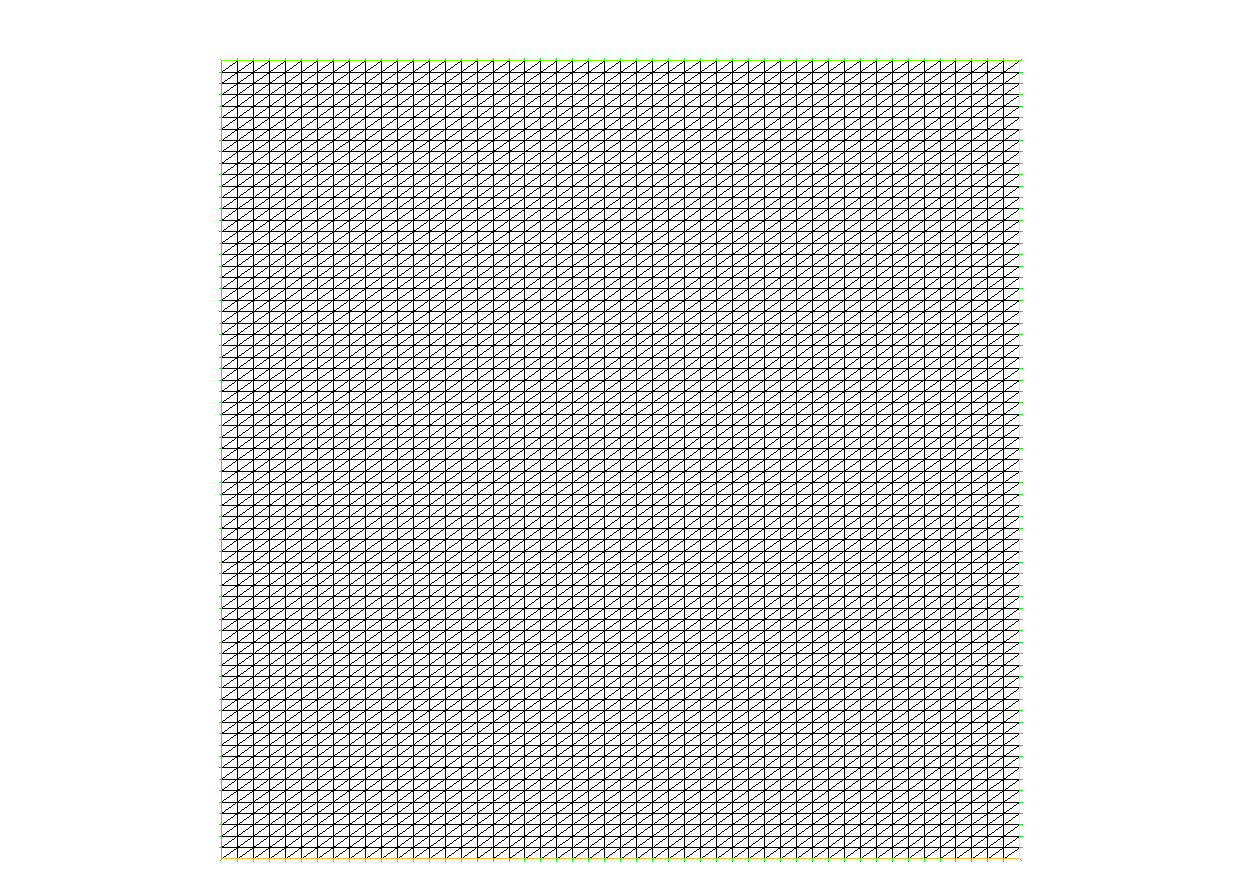
\includegraphics[scale=0.85]{maillage-eps-converted-to.pdf}\\
\caption{Maillage triangulaire d'un carré}
\label{mail1}
\end{figure}

Pour tout entier $k\geq 1$, on appelle treillis d'ordre $k$ l'ensemble :\\
\begin{equation*}
\Sigma_{k}=\left\{ x\in K \text{ tel que } \lambda_{j}\left(x\right)\in\left\{0, \frac{1}{k},...,\frac{k-1}{k}, 1\right\} \text{ pour }1\leq j\leq N\right\}
\end{equation*}
Avec $\lambda_{j}$ les coordonnées barycentriques de $x\in\mathbb{R}^{N}$ définies par:\\
\begin{equation*}
\sum_{j=1}^{N+1}\lambda_{j}=1 \;\;\;\sum_{j=1}^{N+1}a_{i,j}\lambda_{j}=x_{i} \texttt{ pour } 1\leq i \leq N
\end{equation*}
Avec les $a_{i,j}$ les sommets de notre maillage.\\

Nous définissons l'ensemble $\mathbb{P}_{k}$ comme les polynômes à coefficients réels de $\mathbb{R}^{N}$ dans $\mathbb{R}$ de degré inférieur ou égal à $k$. L'intérêt de ces notions est qu'un treillis $\Sigma_{k}$ d'un maillage $K$ permet de caractériser tous les polynômes de $\mathbb{P}_{k}$. On dit alors que $\Sigma_{k}$ est $\mathbb{P}_{k}$ unisolvant.On note les points du treillis $\Sigma_{k}$  $\left(\sigma_{j}\right)_{1\leq j\leq n_{k}}$. Il existe donc une base $\left(\psi_{j}\right)_{1\leq j\leq n_{k}}$ de $\mathbb{P}_{k}$ telle que :$\psi_{j}\left(\sigma_{i}\right)=\delta_{ij}$  $1\leq i, j\leq n_{k}$\\

On définit les noeuds de liberté comme l'ensemble des points $\left(\hat{a}_{i}\right)_{1\leq i\leq n_{d_{l}}}$ des treillis d'ordre $k$. On ne compte que'une seule fois les points qui se trouvent dans plusieurs de nos treillis. $n_{d_{l}}$ est le nombre de degrés de liberté de la méthode des éléments finis $\mathbb{P}_{k}$. On définit le sous-espace $V_{0h}$ comme ci-dessous :\\
\begin{align*}
V_{0h}=\left\{v\in V_{h} \text{ tel que } v=0 \text{ sur } \partial\Omega\right\}
\end{align*}

L'espace $V_{h}$  est un sous-espace de $H^{1}\left(\Omega\right)$ dont la dimension vaut le nombre de degrés de liberté et est donc finie. Il existe une base de $V_{h}$ qu'on nommera $\left(\phi_{i}\right)_{1\leq i\leq n_{d_{l}}}$ qu'on définit de la manière suivante : $\phi_{i}\left(\hat{a}_{j}\right)=\delta_{ij}$  $1\leq i, j\leq n_{d_{l}}$ telle qu'on ait :
\begin{equation*}
v(x)=\sum_{i=1}^{n_{d_{l}}}v\left(\hat{a}_{i}\right)\phi_{i}\left(x\right)
\end{equation*}

Revenons à notre exemple. Résoudre ce système par la méthode des éléments finis revient à trouver $u_{h}\in V_{0h}$ tel que
\begin{equation*}
\int_{\Omega}\nabla u_{h}.\nabla v_{h}dx=\int_{\Omega}fv_{h}dx \;\; \forall v_{h}\in V_{0h}
\end{equation*}
Ce qui équivaut à l'expression ci-dessous après avoir décomposé $u_h$ dans notre base et en prenant $v_{h}=\phi_{i}$
\begin{equation*}
\sum_{j=1}^{n_{d_{l}}}u_h\left(\hat{a}_{j}\right)\int_{\Omega}\nabla\phi_{j}.\nabla\phi_{i}dx=\int_{\Omega}f\phi_{i}dx
\end{equation*}
On introduit la matrice de rigidité $\mathcal{K}_{h}$ définie par:
\begin{align*}
\mathcal{K}_{h}=\left(\int_{\Omega}\nabla\phi_{j}.\nabla\phi_{i} dx\right)_{1\leq i, j\leq n_{d_{l}}}
\end{align*}
On obtient alors le système linéaire : $\mathcal{K}_{h}U_{h}=b_{h}$ avec
\begin{align*}
U_{h}=\left(u_{h}\left(\hat{a}_{j}\right)\right)_{1\leq j \leq n_{d_{l}}} \;\; b_{h}=\left(\int_{\Omega}f\phi_{i}dx\right)_{1\leq i\leq n_{d_{l}}}
\end{align*}
\subsection{Exemple de la méthode des éléments finis}
Soit le problème suivant :
\begin{align*}
\left\{\begin{matrix}
-\Delta\left(u\right)=f,  u\in\Omega\\
u=0 \texttt{ sur }\Gamma
\end{matrix}
 \right.
\end{align*}
\subsubsection{Formulation variationnelle de notre problème}
Comme nous avons vu ce problème peut se mettre sous la forme suivante :
\begin{align*}
\forall v\in V a(u,v)=L(v)
\end{align*}
avec
\begin{equation*}
a(u,v)=\int_{\Omega}\nabla u.\nabla v
\end{equation*}
\begin{equation*}
L(v)=\int_{\Omega}fv
\end{equation*}
\begin{equation*}
V=H_{0}^{1}=\left\{v\in L^{2}\left(\Omega\right), \nabla u\in L^{2}\left(\Omega\right), v=0 \texttt{ sur }\Gamma\right\}
\end{equation*}
Montrons que le théorème de Lax-Milgram s'applique.
Est-ce que notre $a(u,v)$ est bien continu ?
\begin{align*}
\lvert a\left( u,v\right)\rvert=\lvert \int_{\Omega}\nabla u.\nabla v dx\rvert\leq \int_{\Omega} \lvert\nabla u.\nabla v\rvert dx \leq \lVert u'\rVert_{L^{2}\left(\Omega\right)}\lVert v'\rVert_{L^{2}\left(\Omega\right)}
\end{align*}
Or
\begin{align*}
\lVert u'\rVert_{L^{2}\left(\Omega\right)}+\lVert u\rVert_{L^{2}\left(\Omega\right)}=\lVert u\rVert_{V}
\end{align*}
D'où :
\begin{align*}
\lvert a\left( u,v\right)\rvert\leq \lVert u \rVert_{V}\lVert v \rVert_{V}
\end{align*}
Donc $a\left(.,.\right)$ est bien une forme bilinéaire continue. Maintenant démontrons qu'elle est $V-$elliptique.
\begin{align*}
a(v,v)=\int_{\Omega}\nabla v.\nabla v=\int_{\Omega} \left(\nabla v\right)^{2}\geq C\times \lVert v\rVert_{V}^{2}
\end{align*}
D'après l'inégalité de Poincaré. Donc notre forme est bien $V-$elliptique. Montrons désormais que $L(v)$ est continue.
\begin{align*}
\lvert L(v)\rvert=\lvert\int_{\Omega}fv\rvert\leq \int_{\Omega}\lvert fv\rvert \leq \lVert f\rVert_{L^{2}(\Omega)}\lVert v\rVert_{L^{2}(\Omega)}\leq C \lVert v\rVert_{V}
\end{align*}
D'après l'inégalité de Cauchy-Schwarz. Donc nous pouvons appliquer le théorème de Lax-Milgram.
\subsubsection{Méthode des éléments finis}
Nous allons désormais approximer notre solution par la méthode des éléments finis. Pour cela nous choisissons de faire notre maillage sur le carré unité avec des triangles $\mathbb{P}_{1}$.\\
Notre treillis $\Sigma_{k}$ est l'ensemble des coordonnées cartésiennes de notre maillage. Prouvons qu'il est $\mathbb{P}_{1}\left(\mathbb{R}^ {2}\right)$-unisolvant.\\
Nous allons travailler sur un des triangles de notre maillage. Nous rappellons ici que $\mathbb{P}_{1}\left(\mathbb{R}^ {2}\right)=vect\left\{1, x, y\right\}$. Pour prouver l'unisolvance nous allons tout d'abord montrer que la dimension de $\mathbb{P}_{1}$ est égal au cardinal de notre treillis. Puis nous allons tenter de démontrer qu'il n'existe qu'une unique fonction telle que $\forall a\in \Sigma_{k}\; p(a)=0\Rightarrow p=0$\\
\begin{align*}
\mathtt{dim}\mathbb{P}_{1}\left(\mathbb{R}^ {2}\right)=\frac{\left(n+k\right)!}{n!k!}=\frac{3!}{2!}=3
\end{align*}
Or $\mathtt{card}\Sigma_{k}=3$ puisque nous avons dans un seul triangle trois sommets. La première partie est donc vérifiée.\\
Soit$a_{1}, a_{2}, a_{3}$ les trois sommets de notre triangle. On sait que toute fonction $p$ peut s'écrire sous la forme $p(v)=a+bx+cy, v\in\mathbb{P}_{1}\left(\mathbb{R}^{2}\right)$.\\
On pose $a_{1}=\begin{pmatrix}
x_{1}\\
y_{1}
\end{pmatrix}
, a_{2}=\begin{pmatrix}
x_{2}\\
y_{2}
\end{pmatrix}
,a_{3}=\begin{pmatrix}
x_{3}\\
y_{3}
\end{pmatrix}$
On obtient alors le système d'équations suivant :\\
\begin{align*}
\left\{\begin{matrix}
p\left(a_1\right)=a+bx_1+cy_1=0\\
p\left(a_2\right)=a+bx_2+cy_2=0\\
p\left(a_3\right)=a+bx_3+cy_3=0
\end{matrix}\right.\Leftrightarrow\left\{\begin{matrix}
a+bx_1+cy_1=0\\
b(x_2-x_1)+c(y_2-y_1)=0\\
b(x_3-x_1)+c(y_3-y_1)=0
\end{matrix}\right.\\
\Leftrightarrow\left\{\begin{matrix}
a+bx_1+cy_1=0\\
b(x_2-x_1)+c(y_2-y_1)=0\\
(x_2-x_1)\left(b(x_3-x_1)+c(y_3-y1)\right)-(x_3-x_1)\left(b(x_2-x_1)+c(y_2-y_1)\right)=0
\end{matrix}\right.\\
\Leftrightarrow\left\{\begin{matrix}
a+bx_1+cy_1=0\\
b(x_2-x_1)+c(y_2-y_1)=0\\
c\left[(x_2-x_1)\times (y_3-y1)-(x_3-x_1)\times(y_2-y_1)\right]=0
\end{matrix}\right.
\end{align*}
Or $(x_2-x_1)\times (y_3-y1)-(x_3-x_1)\times(y_2-y_1) \neq 0$. En effet, cela représente le double de l'aire de notre triangle. Elle ne peut pas \^etre nulle car sinon nos trois points seraient alignés. Donc $c=0$\\
De plus nous avons le système suivant en soustrayant nos équations de départ :
\begin{align*}
\left\{\begin{matrix}
b(x_1-x_2)=0\\
b(x_2-x_1)=0\\
b(x_3-x_1)=0
\end{matrix}\right.
\end{align*}
Or il est impossible que $x_1=x_2=x_3$ donc obligatoirement $b=0$ On déduit alors aisément que $a=0$. Nous avons donc prouvé que notre treillis était $\mathbb{P}_1\left(\mathbb{R}^2\right)-$unisolvant.\\

Comme nous avons vu précédemment, il est alors possible de mettre notre équation sous la forme d'un système linéaire : $\mathcal{K}_{h}U_{h}=b_{h}$. Par exemple, si on prend $f$ égal à 0.001, on obtient :
\begin{align*}
\mathcal{K}_{h}=\left(
\begin{matrix}
4  &    -1    &  0   &   -1    &  0  &    0   &   0  &    0  &    0\\
-1   &   4  &    -1  &    0     & -1  &    0  &    0  &    0  &    0\\
0    &  -1    &  4   &   0    &  0   &   -1 &     0   &   0 &     0\\
-1  &    0   &   0    &  4   &   -1 &     0   &   -1  &    0  &    0\\
0  &    -1   &   0   &   -1  &    4    &  -1  &    0   &   -1  &    0\\
0   &   0  &    -1   &   0   &   -1  &    4   &   0  &    0  &    -1\\
0   &   0   &   0   &   -1    &  0    &  0  &    4   &   -1   &   0\\
0    &  0    &  0   &   0    &  -1    &  0   &   -1  &    4    &  -1\\
0    &  0  &    0   &   0    &  0   &   -1   &   0    &  -1   &   4\\
\end{matrix}\right)
\end{align*}
\begin{align*}
b_h =\left(
\begin{matrix}
6.25\times 10^{-5}\\
\vdots\\
6.25\times 10^{-5}
\end{matrix}\right)
\end{align*}
Nous pouvons alors résoudre notre système.
